\chapter{Marco Teórico}

%
% Parte conceptual
%

\section{Normatividad}

De acuerdo con la Real Academia de la Lengua Española, un \textbf{reglamento} es una norma que rige la organización y funcionamiento de cualquier establecimiento o institución, públicos o privados. \parencite{rae}

\subsection{Marco Jurídico y Marco Normativo}

A continuación se definen los siguientes conceptos.

\begin{quote}
\textbf{Marco Jurídico}: Conjunto de leyes, reglamentos, Conjunto de disposiciones, leyes, reglamentos y acuerdos a los que debe apegarse una dependencia o entidad en el ejercicio de las funciones que tienen encomendadas.. \parencite{riverarobles}
\end{quote}

\begin{quote}
% Change this definition
\textbf{Marco Normativo}: Conjunto general de normas, criterios, metodologías, lineamientos y sistemas, que establecen la forma en que debe desarrollarse su cumplimiento. \parencite{diccionariomarconormativo}
\end{quote}

Para que un reglamento deba ser válido debe tener una base legal y establecer las especificaciones del cumplimiento. Ambos conceptos de marco jurídico y normativo se fundamentan en la necesidad de una base para la regulación de las actividades que se desempeñan de manera colectiva y a nivel individuo.

La unidad atómica de un hecho que establece un enunciado legal es el \textit{artículo}, expresando mediante la misma información de un concepto de manera especifica. Es por esto que estos enunciados forman la base para fundamentar un derecho u obligación. Así mismo, los artículos se dividen de manera estructural agrupando temas de una sola materia.

\subsection{Reglamentos del Instituto Politécnico Nacional}

Como ya se ha mencionado, \textit{el Instituto Politécnico Nacional es un órgano desconcentrado de la Secretaría de
Educación Pública}, que a su vez es una dependencia del gobierno del estado. El IPN tiene su base jurídica a través de su \textit{Ley Orgánica} para regular las funciones científicas y académicas que debe cumplir.

A continuación se muestra una tabla con los 29 reglamentos utilizados en el marco normativo del Instituto Politécnico Nacional y una descripción de la materia normativa que abarca.

\newpage

\begin{tabular}{ | m{17em} | m{25em}|}
    \hline
    \textbf{Reglamento} & \textbf{Descripción} \\
    \hline
    Reglamento de Estudios de Posgrado & Norma el ingreso, permanencia y egreso de los alumnos que cursen alguno de los programas académicos  de  nivel  posgrado, \\
    \hline
    Reglamento Orgánico & Establece  las  bases  de la organización y la distribución de competencias entre las distintas unidades administrativas, académicas y otras dependencias que conforman la estructura orgánico-funcional. \\
    \hline
    Reglamento del Sistema de Becas por Exclusividad & Establece las condiciones y términos para el otorgamiento de becas por exclusividad en el ámbito de competencia para profesores de carrera de tiempo completo clasificado como trabajador base y a los incorporados a través del Programa de Contataciones Extraordinarias. \\
    \hline
    * Reglamento Interior de la Comisión Nacional del Sistema de Ahorro para el Retiro & Define la organización, estructura y facultades de las unidades administrativas de la Comisión Nacional  del  Sistema  de  Ahorro  para  el  Retiro.\\
    \hline
    * Reglamento del Instituto para la Protección al Ahorro Bancario & Establece las unidades administrativas del Instituto para la Protección al Ahorro Bancario. \\
    \hline
    * Reglamento de la Ley sobre Refugiados y Protección Complementaria & Establece las condiciones de refugiado y reglamenta las sus leyes de protección. \\
    \hline
    *Reglamento para la integración y funcionamiento de la Comisión de Apelación y Arbitraje del Deporte & Regular la integración y funcionamiento de la Comisión de Apelación y Arbitraje del Deporte. \\
    \hline
    *Reglamento de la Junta de Gobierno del Consejo Nacional para Prevenir la Discriminación. & Reglamenta la conducción y funcionamiento de la Asamblea Consultiva del Consejo Nacional para Prevenir la Discriminación. \\
    \hline
    * Reglamento de Pasaportes y del Documento de Identidad y Viaje. & Regular la expedición, renovación y cancelación del pasaporte y del documento de identidad y viaje. \\
    \hline
    Reglamento General de Estudios del Instituto Politécnico Nacional. & Establecer las condiciones que regulan el ingreso, la trayectoria escolar, la permanencia y el egreso de alumnos que cursen algún programa académico de los niveles medio superior, superior y posgrado, así como de los usuarios de todos aquellos programas que se ofrezcan.  \\
    \hline
    Reglamento de promoción docente del Instituto Politécnico Nacional. & Regula el proceso de promoción docente. \\
    \hline
    *Reglamento de Becas del Programa de Fomento, Formación, Desarrollo y Vinculación de Recursos Humanos de Alto Nivel del Consejo Nacional de Ciencia y Tecnología. &  Para las instancias encargadas de la conducción y operación del Programa  de Fomento, Formación, Desarrollo y Vinculación de Recursos Humanos de Alto Nivel del CONACyT y para quienes estén recibiendo o pretendan recibir los apoyos o beneficios. \\
    \hline
    Reglamento de Integración Social del Instituto Politécnico Nacional. & Regula las actividades de integración social, sus alcances y objetivos. \\
    \hline
    Reglamento del Consejo General Consultivo del Instituto Politécnico Nacional. & Regular la integración, funcionamiento y organización del Consejo General Consultivo del Instituto Politécnico Nacional. \\
    \hline
    Reglamento del Decanato del Instituto Politécnico Nacional. & Regular el funcionamiento y atribuciones del Decanato como órgano colegiado, de su presidente y de los maestros decanos de cada escuela, centro o unidad de enseñanza y de investigación del Instituto. \\
    \hline
    Reglamento del Archivo Histórico del Instituto Politécnico Nacional. & Otorgar distinciones por el reconocimiento que hace la comunidad politécnica a una conducta, trayectoria, servicios o acciones ejemplares o sobresalientes que hayan tenido por objeto exaltar el prestigio de esta casa de estudios, apoyar la realización de sus finalidades, impulsar el desarrollo de la educación técnica en el país o beneficiar a la humanidad. \\
    \hline
    
\end{tabular}

\begin{tabular}{ | m{17em} | m{25em}|}
    \hline
    \textbf{Reglamento} & \textbf{Descripción} \\
    \hline
    Reglamento de Distinciones al Merito Politécnico del Instituto Politécnico Nacional. &  Fijar las relaciones entre el personal docente de Educación Media Superior y de Educación Superior del Instituto Politécnico Nacional y el Programa de Estímulo al Desempeño Docente. \\
    \hline
    Reglamento del Programa de Estímulo al Desempeño Docente del Instituto Politécnico Nacional. & Fijar las relaciones entre el personal docente de Educación Media Superior y de Educación Superior del Instituto Politécnico Nacional y el Programa de Estímulo al Desempeño Docente. \\
    \hline
    Reglamento Interno del Instituto Politécnico Nacional. & Establecer lineamientos metodológicos básicos de la reforma reglamentaria el mantener y respetar estrictamente lo establecido en la Ley Orgánica. \\
    \hline
    Reglamento Interior de la Comisión de Operación y Fomento de Actividades Académicas del Instituto Politécnico Nacional. & Establecer los reglamentos  para el cumplimiento del objetivos del COFAA como Organismo Público Descentralizado y Entidad  de  la  Administración  Pública  Paraestatal. \\
    \hline
    Reglamento de Titulación Profesional del Instituto Politécnico Nacional. & Establecer las normas para el otorgamiento de títulos profesionales a los pasantes del Instituto Politécnico Nacional y de sus planteles incorporados.  \\
    \hline
    Reglamento de Evaluación del Instituto Politécnico Nacional. & Regular  la  función  de  evaluación  que  se  desarrolla  en  el  Instituto  Politécnico  Nacional. \\
    \hline
    Reglamento de Academias del Instituto Politécnico Nacional. & Establecer normas para la integración y funcionamiento de las academias de profesores en las escuelas,  centros y unidades de enseñanza. \\
    \hline
    Reglamento de Planeación del Instituto Politécnico Nacional. & Establecer las normas y principios básicos para la integración y funcionamiento del Sistema Institucional de Planeación. \\
    \hline
    Reglamento de Prácticas y Visitas Escolares del Instituto Politécnico Nacional. & Establecer las normas a las que se sujetarán las prácticas o visitas escolares que realicen los alumnos y pasantes del IPN. \\
    \hline
    Reglamento de las Condiciones Generales de Trabajo del Personal no Docente del Instituto Politécnico Nacional. &  Fija las Condiciones de Trabajo del Personal No Docente del Instituto Politécnico Nacional, que conjuntamente con sus dos anexos. \\
    \hline
    Reglamento del Patronato de Obras e Instalaciones del Instituto Politécnico Nacional. & Establece las normas a las que se sujetan el Patronato de Obras e Instalaciones del Instituto Politécnico Nacional como órgano público descentralizado. \\
    \hline
    Reglamento de las Condiciones Interiores de Trabajo del Personal Académico del Instituto Politécnico Nacional. &  Fija las condiciones de trabajo del personal académico del Instituto Politécnico Nacional. \\
    \hline
    Reglamento del Centro Nacional de Cálculo. & Establece las normas para los procesos profesionales y actividades de investigación del Centro Nacional de Cálculo. \\
    \hline
\end{tabular}

%
% Parte conceptual
%

\section{Inteligencia Artificial}

La inteligencia artificial es un conjunto multidisciplinario de ciencias y filosofías basados en el principio de la simulación de la inteligencia humana, la mas compleja observada hasta ahora. Abarca una variedad amplia de aspectos que podrían considerarse dentro de un \textit{comportamiento mediante el razonamiento}, tales como maquinas que se conduzcan solas o algoritmos que puedan optimizar decisiones basadas en pronósticos obtenidos mediante aprendizaje. \parencite{russelnorvig}.

Los algoritmos que implementan esta inteligencia añaden mas valor cuando intentan asimilar una función desconocida para poder acercarse a un comportamiento que reproduzca esos resultados. A esto se le conoce como \textbf{aprendizaje automático} y generalmente se dividen en dos categorías: \textit{supervisado} y \textit{no supervisado}. \parencite{murphypkevin}

% \subsection{Aprendizaje Automático Supervisado}

% Esta forma de aprendizaje está basada en el enfoque predictivo basado en el estado de la entrada a una función. Esto requiere construir un modelo mediante una población de datos de entrada y otra población de datos que implican que fueron obtenidos a base de la entrada. El objetivo es poder mapear una entrada $\mathbf{x}$ a una salida $y$, dado un conjunto de datos de entrenamiento en forma de tupla entrada-salida:

% $$
% D = \{\mathbf{x_i}, y_i\}^N_{i=1}
% $$

% La figura \ref{fig:iris-classification} muestra como se clasifican tipos de flores iris de acuerdo usando \textit{machine learning}. De esta forma se busca encontrar un modelo de clasificación que esté en función de los atributos de la entrada.

% \begin{figure}[ht]
%     \centering
%     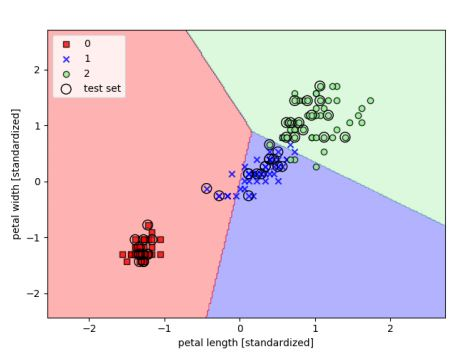
\includegraphics[scale=0.75]{images/2/iris-classification}
%     \caption{Clasificación un conjunto de datos de flores iris.}
%     \label{fig:iris-classification}
% \end{figure}

% \subsection{Algoritmo K-Means}



% Esto es especialmente útil en aplicaciones como chatbots porque queremos que \textbf{la intención del usuario esté en función del mensaje que escribe}. Por ejemplo, algunas intenciones y ejemplos de mensajes son:

% \begin{itemize}
%     \item \textbf{Saludar}:
    
%     \begin{enumerate}
%         \item \textit{Hola.}
%         \item \textit{Buenos días.}
%         \item \textit{Buenas tardes.}
%     \end{enumerate}
    
%     \item \textbf{Solicitar Reglamento}
    
%     \begin{enumerate}
%         \item \label{itm:intencion-solicitar}\textit{Dime qué dice el \textbf{artículo 3} de la \textbf{Ley Orgánica}}.
%         \item \textit{¿Qué dice el \textbf{artículo 9} del \textbf{Reglamento General de Estudios}?}
%     \end{enumerate}
% \end{itemize}

% La idea es que con base a un conjunto de entrenamiento de mensajes ejemplo podamos \textit{clasificar la intención}. Además, una vez identificada la intención también pueda clasificar a \textbf{entidades} de interés para saber qué información se está solicitando. Por ejemplo, el ejemplo \ref{itm:intencion-solicitar} de la intención de solicitar reglamento requiere reconocer que se está pidiendo el \textbf{artículo} un \textbf{documento}, por lo que son dos entidades que el chatbot debe aprender en ese ejemplo. 

% Cuando se trata de texto, por lo regular se utilizan \textbf{redes neuronales recurrentes}, que aprenden con base a una secuencia de valores.

\section{Procesamiento de lenguaje natural}

El lenguaje natural es un fenómeno lingüístico que abarca la creación y constante evolución del lenguaje que los humanos obtienen a través del uso ordinario y cotidiano en el uso de la comunicación formal. El lenguaje natural es la forma mas sencilla en la que se codifica conocimiento a través de hábitos cognitivos pero a la vez complejo debido a que la inteligencia humana no tienen forma estructurada de comprenderse.

El procesamiento de lenguaje natural, también conocido como \textit{lingüística computacional}, es una aplicación de la inteligencia artificial enfocada a crear entidades que puedan simular la inteligencia humana con capacidades de entendimiento y síntesis de lenguaje natural o humano. La \textit{lingüística} es el estudio científico del lenguaje que se encarga de estudiar múltiples aspectos del lenguaje y funciona como una base estructurar elementos de un lenguaje en componentes o unidades dependiendo el tipo de análisis.

Uno de las unidades mas comunes es una \textbf{palabra} la cual puede derivar significado por si solo. Posteriormente, existen categorías para clasificar palabras, como lo son \textit{sustantivos}, \textit{verbos}, \textit{adjetivos}, \textit{adverbios}, entre otras menos comunes. \parencite{dipanjan}.

Estas palabras forman grupos para agregar significado mediante \textit{frases} o \textit{cláusulas}, que a su vez pueden estructurarse mediante gramáticas que describan las relaciones entre esos grupos de palabras. Para propósitos de este proyecto, inicialmente tomaremos al conjunto de palabras en oraciones para derivar un significado.

\subsection{Semántica}

Entre los objetos de estudio de la lingüística está la \textbf{semántica}, la cuál envuelve el estudio del \textit{significado}. Por sí solo, la semántica es una teoría compleja que abarca cuestiones un tanto filosóficas y hasta metafísicas, no tanto del significado mismo de las palabras sino la causa del \textit{por qué las palabras tienen significado}. Teorías de la semántica deben contestar las preguntas de \textit{cuál es la naturalez del significado} o \textit{qué produce en nuestro conocimiento cuando conocemos un significado de una palabra} \parencite{sep-word-meaning}.

Para poder procesar significado, se puede subdividir en dos categorías para entender sus componentes \parencite{dipanjan}. Estas son:

\begin{itemize}
    \item \textbf{Semántica léxica}: El estudio del significado de las palabras y símbolos usando morfología y sintaxis.
    \item \textbf{Semántica composicional}: Estudia las relaciones entre las palabras y la combinación de las mismas que constituyen un significado a través de frases y oraciones.
\end{itemize}

Mientras que un ser humano tiene la capacidad de procesar significado de una manera casi inmediata,  resulta ser complejo representar un proceso de \textit{extracción de significado} para una computadora. Hasta la fecha estos problemas solo pueden ser resueltos delimitando el dominio del lenguaje a un uso específico y utilizando \textit{modelos de aprendizaje automático supervisados}, los cuáles obtienen como datos de entrenamiento un grupo de palabras y meta información y otro grupo del "significado representativo que deben tener". Esta abstracción debe poder cuantificarse de alguna manera para poder procesarlo y automatizarlo mediante inteligencia artificial.

Una de las formas mas básicas de representar semántica uniforme es utilizando \textbf{lemas} o \textbf{lematización de palabras}. Un lema es una forma canónica de las palabras. Forma una unidad base para derivar significado dependiendo de las múltiples inflecciones de le base. Un ejemplo común de esto es la conjugación de verbos.

\subsection{Sistemas de Recuperación de Información de Texto}

Regularmente, mucha de nuestra información en el lenguaje español se transmite y se almacena en algún formato textual (e.g., libros, revistas, diccionarios, artículos, publicaciones, conversaciones, etc.). Todo eso se puede almacenar en un repositorio de información para un uso posterior. A esto se le conoce como \textbf{corpus de texto} Pero por si solo, el texto no es suficiente para ser de alguna utilidad, sino lo que significa todo o alguna porción del texto. Entre mas grande crece el corpus de texto, mas dispersa se vuelve la información y mas significado se puede sacar de manera acumulada.

Una de las aplicaciones útiles del procesamiento de lenguaje natural es precisamente el utilizado en este proyecto: la \textbf{recuperación de información} o \textbf{information retrieval} en inglés. La recuperación de información se define como un actividad de obtención de información relevante de una fuente de datos. Estos sistemas son muy útiles debido a que una información relacionada, que puede significar lo mismo o estar muy relacionado pero varía en morfología, e incluso hasta de idioma. Para propósitos de este proyecto, haremos nuestro enfoque la información textual en español para poder dar solución al problema establecido en el capítulo 1.

La forma en que esta recuperación se lleva a cabo es un caso de estudio en su propia cuenta. Puede ser desde la búsqueda idéntica de valores hasta métodos probabilísticos que infieren una similitud semántica de la información. Generalmente estos métodos utilizan una \textbf{función de similitud}, la cual opera sobre un \textbf{espacio vectorial} que contiene información textual. La transformación de un palabra o conjunto de palabras a un vector de palabras se le conoce como \textbf{word embedding} (incrustación de palabras). Mediante esta representación vectorial es posible cuantificar que tan parecidos son dos vectores de palabras o \textit{word embeddings}. \parencite{zhaimassung}.

\begin{figure}[ht]
    \centering
    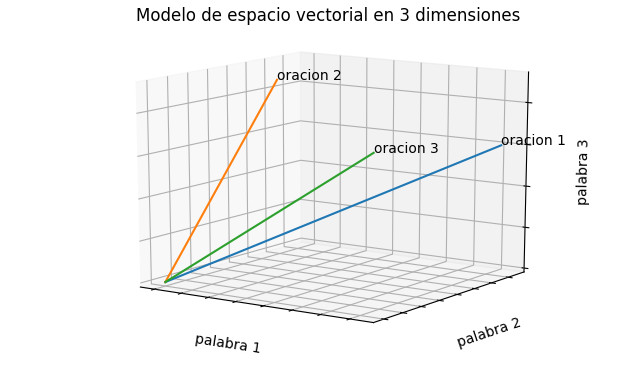
\includegraphics[scale=0.6]{images/2/vector-space-model}
    \caption{Representación gráfica de un vocabulario de 3 palabras sobre un espacio vectorial de $\mathbb{R}^3$.}
    \label{fig:espacio-vectorial}
\end{figure}

La dimensión de este espacio vectorial es determinada por el tamaño del conjunto en el vocabulario de palabras que se usarán en un modelo lingüístico. La figura \ref{fig:espacio-vectorial} muestra un ejemplo de un espacio vectorial de 3 dimensiones con las que se pueden construir oraciones; los vectores en la gráfica son oraciones y se les conoce como \textbf{vectores de palabras}. Bajo esta representación vectorial se pueden ejecutar operaciones matemáticas para cuantificar qué tan similar son estas oraciones en el espacio.

Por ejemplo, si la entrada es una consulta transformada a un vector de palabras $\vec{q}$ buscaremos trasladar esta consulta en el espacio vectorial y observar qué vectores cercanos se encuentran al de la consulta; entre mas cercanos, mas relevantes serán. Una función de similitud entre vectores muy conocida es la \textbf{similitud coseno}. 

Sean 

$$\vec{a},\vec{b} : \text{vector de } n \text{ dimensiones correspondiente a una oración.}$$

Entonces, la similitud entre esas dos oraciones se puede calcular mediante la fórmula:

$$
sim(\vec{a}, \vec{b}) = \frac{\vec{a} \dot \vec{b}}{\| \vec{a} \| \| \vec{b} \|}
$$

Estos vectores se pueden construir de múltiples maneras: mediante usos de aprendizaje automático representados como $\vec{w} = (w_0, w_1, ..., w_n)$ en donde $w_i$ pertenece a un vocabulario $\mathbf{V}$. Algunas formas de representación de vectores son:

\begin{itemize}
    \item \textbf{Representación de bits}: una forma sencilla y rápida de representar un conjunto de palabras es indicando si esa palabra está presente o no. Matemáticamente, el vector se calcula de la siguiente manera:
    
    \begin{equation*}
        a(i) = 
        \begin{cases}
            1 & \text{si la palabra está presente en la oración}\\
            0 & \text{en otros casos}
        \end{cases}
    \end{equation*}

    \item \textbf{Representación basados en frecuencias}: Dada una colección de documentos se puede utilizar varios factores para determinar significado de un conjunto de palabras en cuánto al dominio de esos documentos, como la frecuencia de las veces que aparece en el documento y en cuántos de ellos aparece. Derivado de eso se puede refinar aún mas normalizando palabras que se utilizan de manera excesiva y destacar palabras poco frecuentes como mas significativas. 
    
    Sea
    
    \begin{align*} 
        q: & \text{ una oración correspondiente a una consulta}\\
        d: & \text{ un documento}\\
        M: & \text{ la cantidad de documentos}\\
        c(w, q): & \text{ función que cuenta las ocurrencias de } w \text{en } q\\
        df(w): & \text{ cantidad de documentos que contienen a } w
    \end{align*}
    
    Entonces una oración cosulta $q$ puede ser representada mediante la siguiente fórmula:

    $$
    f(q, d) = \sum_{w \in q \cup d} c(w, q) c(w, d) log \frac{M + 1}{df(w)},
    $$
\end{itemize}

\subsection{Algoritmo de Detección de Paráfrasis}
\label{sec:deteccion-parafrasis}

Para este proyecto usaremos un método llamado detección de paráfrasis, el cual consiste en buscar una forma de relacionar las palabras utilizadas en la consulta y obtener los segmentos de texto en los reglamentos del marco normativo. De esta manera evitamos búsquedas de palabras exactas cuando podrían encontrarse como un sinónimo. Este algoritmo fue presentado por \cite{fernando2008semantic}.

En primera instancia, se debe considerar un espacio vectorial que abarque la mayor cantidad de palabras posibles, pero entrenando su semántica lo mas cercano posible al tema o dominio de interés. Por ejemplo, \textbf{Spacy} proporciona un modelo entrenado utilizando el algoritmo \textbf{word2vec} (\url{https://github.com/explosion/spacy-models/releases/tag/es_core_news_md-2.2.5}) para el lenguaje español. 

Una vez obtenido este espacio, se debe representar las palabras en su forma vectorial y utilizar la similitud coseno para construir una matriz $\mathbf{W}$, la cuál representa todas las similitudes posibles que existen en el vocabulario. Cabe mencionar que la matriz resultante es una matriz cuadrada cuya condición $\mathbf{W}_{i,j} = 1$ cuando $i = j$; es decir, una palabra es similar a sí misma.

$$
\mathbf{W}_{i,j} = sim(w_i, w_j)
$$

Supongamos entonces que un usuario introduce una consulta $\vec{q}$, la cuál es una oración compuesta de palabras utilizando el mismo vocabulario. Queremos comparar esta consulta con segmentos de texto $\vec{s}$ para calcular su relevancia. Esto se hace con la siguiente fórmula:

$$
sim(\vec{q}r, \vec{s}) = \frac{ \vec{q^T} \mathbf{W} \vec{s}}{\| \vec{q} \|  \| \vec{s} \|}
$$

Los vectores $\vec{q}$ y $\vec{s}$ son vectores binarios indicando la presencia de una palabra. Como cada palabra constituye una dimensión en este espacio vectorial, estos vectores debemos representarlos como la suma de los vectores unitarios que representan las palabras presentes en la oración. Si $\vec{a}$ se obtiene a partir de una oración, entonces a se obtiene de la siguiente forma:

$$
\vec{a} = 
\begin{pmatrix}
    a_0\\
    a_1\\
    a_2\\
    \vdots \\
    a_n
\end{pmatrix}
$$

\begin{equation*}
a(i) = 
    \begin{cases}
        1 & \text{si la palabra está presente en la oración}\\
        0 & \text{en otros casos}
    \end{cases}
\end{equation*}

Esto hace que solo se calculen las similitudes de las palabras presentes en la consulta y en el texto a comparar, mientras que se ignorar palabras que no están presentes.\textbf{}

\subsection{Preparación de los datos}

Para poder operar consultas con este método, necesitamos lo siguiente:

\begin{enumerate}
    \item Los vectores de las palabras deberán remover \textit{palabras vacías} (artículos, pronombres, preposiciones, etc.).
    \item Las palabras resultantes utilizarán en su forma \textit{lematizada}.
    \item \label{itm:matriz-w} La matriz de similitud $\mathbf{W}$ deberá estar calculada previamente.
\end{enumerate}

\subsection{Métricas Adicionales de Semántica}

El uso exclusivo de una matriz de similitud considera un nivel básico de parafraseo por la mera presencia de palabras en un enunciado, o en su defecto algunas similares. Sin embargo, hay algunos factores adicionales que agregan sentido estructural en cuanto a como se relacionan los conceptos. \parencite{batetsanchesvalls2010semantic}

\begin{figure}
    \centering
    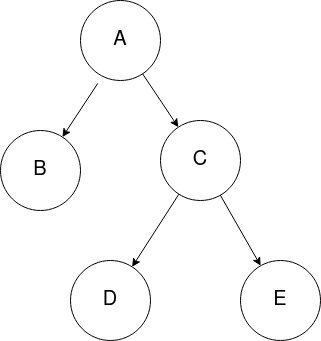
\includegraphics[scale=0.5]{images/2/arbol-simple}
    \caption{Arbol de entidades. Cada nodo representa una entidad mientras que los vértices representan relaciones entre ellos.}
    \label{fig:arbol-entidades}
\end{figure}


Se puede medir el nivel de cercanía en una estructura taxonómica basada en clases ontológicas de su significado. Por ejemplo, agregar una jerarquía de entidades como \textbf{PERSONA} derivando a \textbf{ESTUDIANTE}, la cual puede tener mas clases dependiendo del dominio que deba especificar. En este caso la estructura resultante sería una similar al de la figura \ref{fig:arbol-entidades} y la distancia implicada es la profundidad.


En ese caso, existe una red semántica de entidades conectadas por vértices que implican una relación entre ellas, las cuales se pueden medir con distancias para denotar similitud:

$$
d(c_1, c_2) = \text{Menor cantidad posible de vértices conectando a } c_1 \text{ y } c_2
$$

La ecuación exacta varía dependiendo de los factores a considerar y de la complejidad que se busca. Varias propuestas se pueden encontrar en \cite{batetsanchesvalls2010semantic}.
